\section{Tensão e liberação }
\index{Música!Tensão}

\subsection{O que é tensão}
Ao escutar uma porção de uma peça musical, percebemos que esta provoca na nossa mente
um sentido de antecipação.
Esta percepção nos conduz, internamente, 
a ter um estado variável entre a tensão (expetativa ou ``tension'' em inglês)
ou um sentido de liberação (resolução, descanso, ou ``release'' em inglês).
Assim podemos descrever à tensão como o 
estado onde sentimos a necessidade de obter uma resolução; e dizer, passar a um estado de liberação.
Em muitas ocasiões o compositor usa este recurso para chamar nossa atenção,
deixando-nos impacientes para obter uma resposta. 
Quanto tempo o compositor vai nos torturar esperando a resposta, 
é uma liberdade criativa de cada artista.

\begin{example}
Um exemplo onde é muito fácil perceber o uso da tensão na música, 
para comunicar estados de animo no espectador, 
pode ser escutado no tema principal da banda sonora do filme ``Jaws'' (Tubarão) 1975,
escrita por John Williams\footnote{Este tema é fácil de achar usando as palavras chave:``Jaws main theme soundtrack''.}.

Ao escutar a peça musical automaticamente entraremos num percorrido que nos leva lentamente,
porem sem pausa, a um estado de tensão e suspense, seguido de um pequeno momento de calma,
que cumpre a função de dar-nos uma falsa sensação de paz,
 para logo nos surpreender com um estado de tensão ainda maior;
finalizando o tema num estado de liberação (calma).
\end{example}

\subsection{Como se modifica a tensão?}

Alguns compositores e artistas dividem a obtenção da tensão, em dois grandes grupos \cite{edmtensionrelease1}:
\begin{itemize}
\item \textbf{Macro-tensão:}
é uma tensão que se trabalha durante um período de tempo longo. 
Onde a tensão vai se acumulando para servir de transição entre uma parte do arranjo para outra;
ou também a tensão pode diminuir ao longo do tempo ate chegar a um ponto de baixa energia.
Normalmente, uma macro-tensão é usada para fazer a transição a uma queda, coro, ponte \cite{edmtensionrelease1}, etc.
\item \textbf{Micro-tensão:}
são  quebras isoladas do padrão, que acontecem de forma pontual ao longo da peça musical, 
como alterações na melodia, breques, acordes não resolvidos, etc. 
Em geral pode se referir a qualquer coisa que altere pontualmente a monotonia da peça musical \cite{edmtensionrelease1}.
\end{itemize}~

O aumento ou a diminuição da tensão na música pode ser promovido por vários fatores; 
sendo que este efeito pode ser pontual ou trabalhado ao longo de uma seção.
para compreender melhor como este aspecto da música  é controlado,
 a continuação são listados alguns dos fatores que contribuem à modificação da tenção:
\begin{itemize}
\item o tom \cite[pp. 3]{wright2012essential},
\item a intensidade (volume) \cite[pp. 3]{wright2012essential},
\item a dissonância \cite[pp. 28-29]{kerman2015listen} \cite[pp. 26]{wright2012essential},
\item o ritmo, 
\item as cadencias nas frases musicais,
\item etc.
\end{itemize}~

Para ter uma ideia mais clara de como estes elementos provocam tensão podemos usar a Tabela  \ref{tab:tensionrelease1}.  
\begin{table}[h]
  \centering
  \begin{tabular}{| p{3cm} || p{3.0cm} | p{3.0cm} |}
   \hline 
   Tipo & Tensão     & Relaxação \\ \hline 
   \hline 
   Tom          & Incremento & Diminuição  \\ \hline
   Intensidade  & Incremento & Diminuição  \\ \hline
   Dissonância  & Incremento & Diminuição  \\ \hline
   Ritmo        & Incremento da velocidade & Diminuição da velocidade \\ \hline
   Cadência     & Final aberto & Final fechado \\ \hline
  \end{tabular}
  \caption{Tensão e relaxação na música.}
  \label{tab:tensionrelease1}
\end{table}
Onde na primeira coluna  vemos a caraterística em estudo,
a segunda coluna nos indica que debemos fazer com essa caraterística para aumentar a tensão,
e a terceira coluna nos indica que devemos fazer com a caraterística para diminuir a tensão;
é dizer aumentar a relaxação.

%%%%%%%%%%%%%%%%%%%%%%%%%%%%%%%%%%%%%%%%%%%%%%%%%%%%%%%%%%%%%%%%%%%%%%%%%%%%%%%%
\begin{example}[Tensão pela mudança do tom:]
A Figura \ref{fig:tension-release-tom-1} mostra como podemos incrementar e diminuir a tensão,
pelo aumento e a diminuição do tom. 
Nos 4 primeiros compassos a tensão cresce com o aumento do tom,
e nos 4 últimos compassos a tensão diminui com a diminuição do tom.
\end{example}
\begin{figure}[!h]
     \centering
     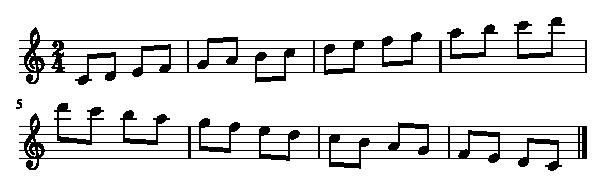
\includegraphics[width=1.0\textwidth]{chapters/cap-musica-topicos/tension-release-tom-1.eps}
     \caption{Incremento e diminuição por mudança do tom.}
     \label{fig:tension-release-tom-1}
\end{figure}


%%%%%%%%%%%%%%%%%%%%%%%%%%%%%%%%%%%%%%%%%%%%%%%%%%%%%%%%%%%%%%%%%%%%%%%%%%%%%%%%
\begin{example}[Tensão pela mudança de intensidade:]
A Figura \ref{fig:tension-release-intensidade-1} mostra como podemos incrementar e diminuir a tenção,
pelo aumento e a diminuição da intensidade. 
Nos 4 primeiros compassos a tensão cresce com o aumento da intensidade,
e nos 4 últimos compassos a tensão diminui com a diminuição da intensidade.
\end{example}
\begin{figure}[!h]
     \centering
     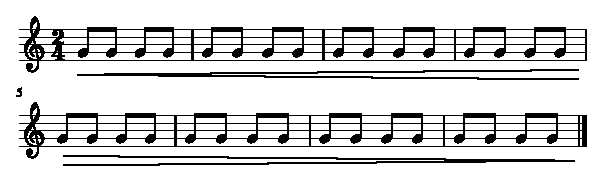
\includegraphics[width=1.0\textwidth]{chapters/cap-musica-topicos/tension-release-intensidade-1.eps}
     \caption{Incremento e diminuição por mudança na intensidade.}
     \label{fig:tension-release-intensidade-1}
\end{figure}


%%%%%%%%%%%%%%%%%%%%%%%%%%%%%%%%%%%%%%%%%%%%%%%%%%%%%%%%%%%%%%%%%%%%%%%%%%%%%%%%
\begin{example}[Tensão pelo uso de dissonâncias:]
A Figura \ref{fig:tension-release-dissonancia-1} mostra como podemos incrementar e diminuir a tenção,
pelo aumento e a diminuição da dissonância. 
Nos 4 primeiros compassos a tensão cresce com o aumento da dissonância,
e nos 4 últimos compassos a tensão diminui com a diminuição da dissonância.
\end{example}
\begin{figure}[!h]
     \centering
     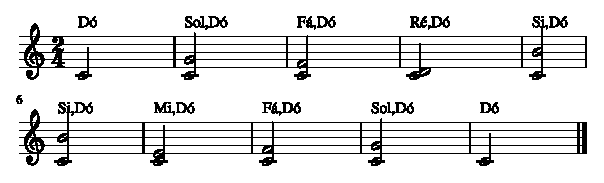
\includegraphics[width=1.0\textwidth]{chapters/cap-musica-topicos/tension-release-dissonancia-1.eps}
     \caption{Incremento e diminuição por mudança na dissonância.}
     \label{fig:tension-release-dissonancia-1}
\end{figure}


%%%%%%%%%%%%%%%%%%%%%%%%%%%%%%%%%%%%%%%%%%%%%%%%%%%%%%%%%%%%%%%%%%%%%%%%%%%%%%%%
\begin{example}[Tensão pela mudança de ritmo:]
A Figura \ref{fig:tension-release-ritmo-1} mostra como podemos incrementar e diminuir a tenção,
pelo aumento e a diminuição da velocidade no ritmo. 
Nos 4 primeiros compassos a tensão cresce com o aumento da velocidade do ritmo,
e nos 4 últimos compassos a tensão diminui com a diminuição da velocidade do ritmo.
\end{example}
\begin{figure}[!h]
     \centering
     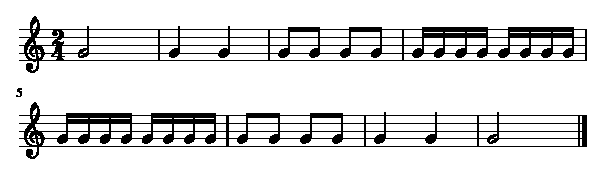
\includegraphics[width=1.0\textwidth]{chapters/cap-musica-topicos/tension-release-ritmo-1.eps}
     \caption{Incremento e diminuição por mudança na intensidade.}
     \label{fig:tension-release-ritmo-1}
\end{figure}

\begin{example}[Tensão pela uso de cadências:]
Para incrementar e diminuir a tenção numa peça musical pelo uso de cadências nas frases musicais,
devemos seguir os tipos de finalizações explicados na Seção \ref{sec:Cadencia}.
Por exemplo, fazendo um paralelo com as frases (gramaticais),
teremos uma expetativa diferente numa frase finalizada de forma enunciativa (``faz frio'') 
que uma frase interrogativa (``Faz frio?''), 
onde a primeira frase nos deixa num estado de relaxação (liberação),
enquanto que a segunda nos deixa uma expetativa (tensão) 
que procura ou espera obter depois uma resposta (resolução).  
\end{example}

% 
% https://www.schoolofcomposition.com/what-is-tension-and-release-in-music/
% https://www.youtube.com/watch?v=613v8nbsWFY
% https://www.youtube.com/watch?v=5kYZmQzMxD0

